\begin{table}[H]
    \centering
	\begin{tabular}{lcccc}
	\textbf{Layer Type} & \textbf{Layer Config} & \textbf{Activation}  & \textbf{Output} & \textbf{Params}\\ \hline
	\conv	& \convKSF{5}{1}{5}	& relu		& \texttt{144,256,5} 	& \texttt{380}\\
	\pool	& \poolN				&	/		& \texttt{72,128,8}		& 0	\\
	\conv	& \convKSF{5}{1}{8}	& relu		& \texttt{72,128,8} 		& \texttt{1008}\\
	\pool	& \poolN				&	/		& \texttt{36,64,12}		& 0	\\	
	\conv	& \convKSF{3}{1}{12}	& relu		& \texttt{36,64,12} 		& \texttt{876}\\
	\pool	& \poolN				&	/		& \texttt{18,32,15} 		& 0	\\
	\conv	& \convKSF{3}{1}{15}	& relu		& \texttt{18,32,15} 		& \texttt{1635}\\
	\pool	& \poolN				&	/		& \texttt{9,16,18}		& 0	\\
	\conv	& \convKSF{3}{1}{18}	& relu		& \texttt{9,16,18} 		& \texttt{2448}\\
	
	\flt		& /					& /			& \texttt{2592}			& \texttt{0}\\
	\dns		& \dnsP{64}			& relu		& \texttt{64}			& \texttt{165952}\\
	\dns		& \dnsP{6}			& softmax	& \texttt{6}				& \texttt{390}\\
	\multicolumn{4}{r}{\textbf{TOTAL}}&{\textbf{172,689}}\\
	\end{tabular}
	%Total params: 172,689
	%Trainable params: 172,689
	%Non-trainable params: 0
\end{table}


\begin{table}[H]
	\centering
	\begin{tabular}{lc}
	\textbf{Param} & \textbf{Value}\\ \hline
	Batch Size 	& 32 \\
	Optimizer 	& Adam \\
	Base lr		& 0.001 \\
	Epochs		& 20 \\
	\end{tabular}
\end{table}


\begin{figure}[H]
	\begin{center}
	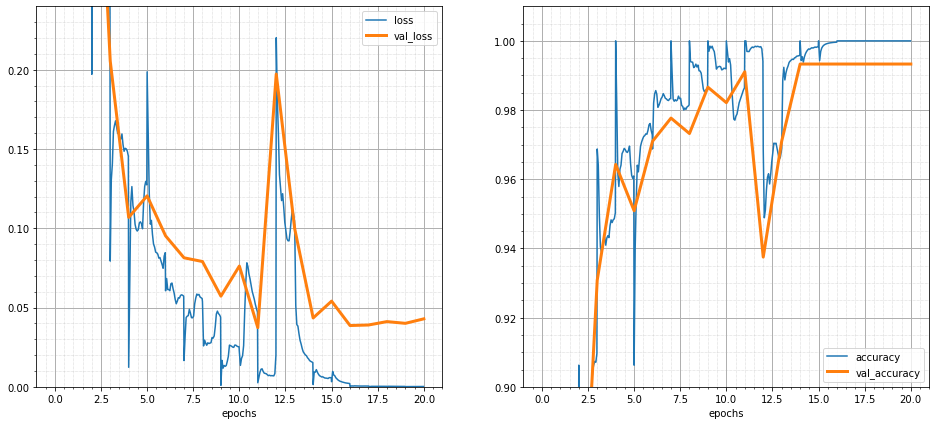
\includegraphics[width=\linewidth]{Immagini/conv-pool-1}
	\caption{Graph of the first run}
	\end{center}
\end{figure}
\begin{table}[H]
	\centering
	\begin{tabular}{cccccc}
		\textbf{Run} &\textbf{Loss}&\textbf{V.Loss} &\textbf{Acc.}&\textbf{V.Acc.}&\textbf{$\Delta$ Acc.} \\ \hline
		1   & 1.8558e-04 &  0.0429  & 1.0000    & 0.9933    & 0.0067\\
		2   & 6.4439e-04 &  0.0461  & 1.0000    & 0.9866    & 0.0134\\
		3   & 1.2224e-04 &  0.0133  & 1.0000    & 0.9933    & 0.0067\\
		\textbf{Avg} & \textbf{3.1740e-04} &  \textbf{0.0341}  & \textbf{1.0000}    & \textbf{0.9911}    & \textbf{0.0893}
	\end{tabular}
\end{table}

This model applies the use of the Conv-Pool technique in order to convolve and reduce the data at every step. Since the reduction is performed by various MaxPooling layers, the first two convolutions have now a stride equal to 1. Pooling helps by reducing the tensor dimension while retaining most of its information. 
Moreover, the model has multiple parameters which are an order of magnitude lower than the previous model. Therefore the model has now little to no overfitting and has gained a good amount of validation accuracy.